\documentclass[conference]{IEEEtran}
\usepackage{graphicx}
\usepackage{multirow}

\usepackage{adjustbox}
\usepackage{algorithm}

\usepackage{algpseudocode}
\usepackage{multirow}

\def\theequation{\arabic{equation}}
\newcommand{\RNum}[1]{\uppercase\expandafter{\romannumeral #1\relax}}
\renewcommand\footnoterule{\hspace{-1em}\rule[0.45em]{\columnwidth}{0.45pt}}
\begin{document}

\title{FedLR: A Federated Learning based Approach for Faster Communication in Edge Environment }

\author{\IEEEauthorblockN{Vipul Singh Negi}
\IEEEauthorblockA{Department of Computer Science and\\Engineering\\National Institute of Technology\\
Rourkela, India 769008\\
vipulhld001@gmail.com}
\and
\IEEEauthorblockN{Suchismita Chinara}
\IEEEauthorblockA{Department of Computer Science and\\Engineering\\National Institute of Technology\\
Rourkela, India 769008\\
suchi.nitrkl@gmail.com}
}



\makeatletter

% \def\ps@IEEEtitlepagestyle{
%   \def\@oddfoot{\mycopyrightnotice}
%   \def\@evenfoot{}
% }
% \def\mycopyrightnotice{
%   {\footnotesize 979-8-3503-0460-2/23/\$31.00~\copyright~2023 IEEE\hfill} % <--- Change here
%   \gdef\mycopyrightnotice{}
% }



% \IEEEoverridecommandlockouts
% \IEEEpubid{\makebox[\columnwidth]{979-8-3503-0460-2/23/23/\$31.00~\copyright2023 IEEE \hfill} \hspace{\columnsep}\makebox[\columnwidth]{ }}

% \makeatletter

% \def\ps@IEEEtitlepagestyle{
%   %\def\@oddfoot{\mycopyrightnotice}
%   \def\@evenfoot{}
% }
% \makeatletter
% \def\footnoterule{\kern-3\p@
%   \hrule \@width 2in \kern 2.6\p@} % the \hrule is .4pt high
% \makeatother
% \newcommand{\copyrightnotice}[1]{{%
%   \renewcommand{\thefootnote}{}% Remove footnote number
%   \footnotetext[0]{#1}%
% }}
\maketitle
% \copyrightnotice{979-8-3503-0460-2/23/\$31.00~\copyright~2023 IEEE}
% \IEEEpubidadjcol

\begin{abstract}
Data are key to the survival of any modern data scenario. With the rise of IoT and Edge Computing, millions of data are shared in a second. The requirement for sound distributed systems is high. One of the best systems is Federated Learning, which works by sharing training parameters rather than training data. This makes it the perfect choice for distributive machine learning. FedAvg is the vanilla algorithm for Federated Learning, but it has a glaring problem of not working correctly for slacker devices. A new approach, FedLR, is proposed in this manuscript to remedy the problem of slacker devices. It provides all the benefits of FedAvg plus it reduces the communication costs as well as creates a fair scenario by also using the slacker devices. The proposed work is compared with FedAvg and FedProx. FedProx is one of the federated learning systems that works for heterogeneous clients while preserving slacker devices. The challenge was to make a fair and communication-efficient strategy for federated learning. It was achieved using FedLR, which uses a time variable to classify devices as slackers and tunes them to handle less data in order to make them contribute to the federation and keep it fair.
\end{abstract}
\begin{IEEEkeywords}
Federated learning, IoT, Deep Learning, Edge Computing
\end{IEEEkeywords}

\IEEEpeerreviewmaketitle



\section{Introduction}
Federated Learning is a new computing technology that promises to provide all the benefits of AI and ML while preserving users' privacy and security. Instead of training on individual users' data, it trains on the client's weight, which is stored locally with the clients'. This system preserves the user's privacy and provides meaningful AI benefits for many applications of distributive computing.Example: WeBankAI \cite{liu2021fate}, Nvidia Clara \cite{nvidia}, and Google Keyboard \cite{yang2018applied}. That does not mean that it does not have any flaws. It is prone to man-in-the-middle attacks and data poisoning, to name a few. Federated Learning is very suitable for IoT and Edge devices as these are well connected to the internet and send vast amounts of data. The Number of connected IoT devices has grown by 13\% in the year 2024, which leads to 18.8 billion global devices \cite{iotana}.\par
Federated Learning provides privacy, scalability, cost-effectiveness, and efficiency. However, each of these features comes at a cost, especially in terms of efficiency. The Federated Learning process is as efficient as its slowest device (slacker), so if someone with older hardware connects to the federation (Fig \ref{fig1}.), the whole system will be bogged down, and the classic FedAvg \cite{mcmahan2017communication} will remove that device from training. So, one of the biggest problems identified is the slacker devices. 


\begin{figure}[htp!]
	\centering
	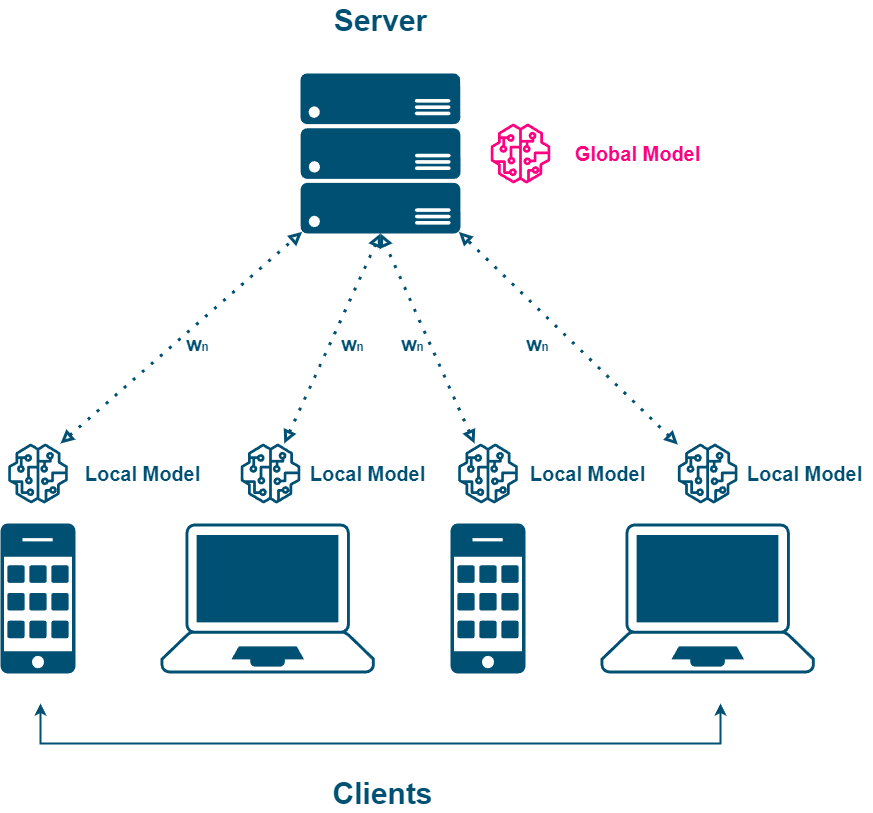
\includegraphics[scale=.25]{Images/FEDLEARN_NEW}
	\caption{Workings of Federated Learning.}
	\label{fig1}
\end{figure}

 In this paper, we present a new strategy which significantly addresses the problem with the old one \cite{mcmahan2017communication}, keeping the effectiveness of federated learning alive. The problem with the vanilla FedAvg is the client selection methodology, which is taken at random, and the device's participation has no threshold value to meet in order to participate in the federated learning process. Another problem with FedAvg is dealing with device heterogeneity, as each device usually tends to have a different CPU, RAM, and GPU, which are the essential blocks of any neural network. FedProx \cite{li2020federated} remedies the heterogeneity of FedAvg to a certain point but doesn't account for fairness. Fairness means all clients should be treated as fair, and their contributions to the global model should carry equal weight. The proposed strategy has been named FedLR, which is a dynamic learning rate and epoch-based client selection strategy.
 
 The proposed work focuses on reducing the total communication time taken by federated learning. Chen et al. \cite{chen2023boosting} used RAM and CPU utilization data from clients in order to boost client selection. But getting such data from clients could lead to device fingerprinting \cite{radhakrishnan2014gtid} \cite{patwari2022dnn}, which puts federated learning at risk.  In this paper, we are employing FedLR, a learning rate based on efficient communication; by considering heterogeneous clients, a time variable has been calculated, and according to that time variable, qualitative decisions towards learning rate selection have been made. In the proposed methodology, a time variable has been calculated, and according to that time variable, qualitative decisions towards learning rate selection have been made.
FedLR guarantees that by considering heterogeneous clients, a time variable has been calculated, and according to that time variable, qualitative decisions towards learning rate selection have been made faster communication time with a fair selection of clients as it always considers slacker devices, which makes this methodology Fair. The main contributions of the proposed work are summarized as follows:
\begin{enumerate}
	\item By conducting extensive sets of experiments we came to a quantitative conclusion about the effects of learning rate ($\eta$) in federated learning which is highly effective parameter in federated learning.
	\item The next contribution is regarding individual clients epochs. The time variable, which represents each client's runtime, is used to find out the slacker devices and adjust the epoch values to reduce the number of slacker devices.
	\item Pairing the time variable with $\eta$ and epoch values of client to perform better client selection which focused on fairness and heterogeneity. A client selection strategy FedLR has been proposed.
\end{enumerate}

The ultimate goal of this work is to present a federated learning approach which reduces the communication cost as well as preserves the Accuracy of the client's model. The remainder of the paper is organized as follows: Section \RNum{2} discusses Related Works. Section \RNum{3} explains the problem statement of the literature. Section \RNum{4} introduces FedLR and explains its key features and how it performs them. Section \RNum{5} does the result and analysis of the proposed algorithm, and Section \RNum{6} finally concludes this paper.


\section{Related Works}
The idea of privacy-preserving deep learning was first presented by Shokri et al. \cite{shokri2015privacy} using distributed and selective SGD to make deep learning models privacy-preserving. After this the Federated learning terminology was coined by McMahan et al. \cite{mcmahan2017communication} in which they proposed the Federate Averaging algorithm and tested it using the MNIST Digit Dataset. The data was partitioned into IID and Non-IID. In Non-IID data, only two-digit data were given to the clients. They have also used CIFAR-10 in the balanced and IID settings. 
\par 
Li et al. \cite{li2020federated} proposed an update to the traditional FedAvg called FedProx by adding statistical heterogeneity (Proximal Term), which handles client heterogeneity better than the previously proposed method.\par Zhang et al. \cite{zhang2024adaptfl} has proposed AdaptFl which is an adaptive FL framework specific to heterogeneous devices. It works on taking the GPU, CPU, Battery, and Network information of the clients. AdaptFl has proposed formulas for calculating energy, transmission, and utilization efficiency. But has the same problem as Chen et al. \cite{chen2023boosting} because taking this much client information will make it vulnerable to device fingerprinting. \par
Zhang et al. \cite{zhang2024fedsl} have proposed FedSL, which uses split layer aggregation and divides the global feature extractor into smaller groups. Then the clients are scored and concatenated back to the original state. \cite{zhang2024fedsl} have considered \cite{mcmahan2017communication} and \cite{li2020federated} as using 100\% of communication cost. \par
Ma et al. \cite{ma2021adaptive} has proposed an adaptive batch sizes FL approach for resource-constrained devices. The test bed uses one workstation as a server and 10 NVIDIA Jetson's as clients. Orlandi et al. \cite{orlandi2023entropy} has proposed an entropy-based FL for Edge intelligence environments and focuses on non-IID data. 19 clients are created using VMs and have been each provided with 4GB of RAM. It calculates entropy and then compares the global mean entropy for each client. The data with lower entropy will be selected for local training; otherwise, it will be discarded. \par 
Mills et al. \cite{mills2023faster} have proposed having a decaying number of local SGD steps, which makes the FL system more efficient. This is also one of the inspirations for the proposed FedLR approach. Mathur et al. \cite{mathur2021device} has implemented federated learning using the Flower framework. They have implemented federated learning in 5 mobile devices (three phones and two tablets). They have used the ever-popular MobileNetV2 \cite{sandler2018mobilenetv2} architecture. Negi et al. \cite{negi2023study} has also studied the same \cite{sandler2018mobilenetv2} architecture for federated learning for FedAvg benchmarking. 
\par  
Hu et al. \cite{hu2025federated} proposed a gradient similarity-based client selection algorithm. It prioritises the clients with similar gradients by calculating cosine similarity. This method will lead to the unfair selection of clients as it doesn't consider slacker devices. Ye et al. \cite{ye2022eco} have proposed Eco-FL, which is much more sustainable than \cite{mcmahan2017communication} and \cite{li2020federated} in terms of energy consumption. \cite{ye2022eco} has also used the flower framework to implement the Eco-FL strategy. \cite{cifar10} and \cite{Krizhevsky09learningmultiple} are used as datasets, and they have tested Eco-Fl in both IID and Non-IID settings. 

\section{Problem Statement}
The FedAvg proposed by \cite{mcmahan2017communication} opened the doors for communication-efficient deep learning networks as they proposed the Federated Averaging methods to train models collaboratively without sharing the underlying training data to preserve the privacy, and ever since then, it has become the state of the art method for Privacy-preserving Deep Learning Models. 
\subsection{Problem Setup} 
The vanilla FedAvg algorithm has some problems when it comes to client selection, heterogeneous computational resources, and fairness, as it focuses primarily on the privacy-preserving aspect of the learning. The algorithm begins with initializing the global model at random or for pre-trained data. This begins the client selection process, which selects clients at random. The global weights are distributed to the clients and the training begins and only stops when we get our desired outcome. To remedy the heterogeneity of FedAvg, a new strategy, FedProx \cite{li2020federated}, was proposed, which tries to contain the dropping slacker devices due to the heterogeneous nature of the devices.

\subsection{Client Selection}

In the vanilla FedAvg, the clients are selected at random using 
\begin{equation}
 m \gets max(C\cdot K,1)
 \label{eq1}
 \end{equation}
where C is the fraction of selected clients and K is the actual clients, which gives us the total number of m clients for the federated learning. This method of selecting clients is good, but it can easily be improved upon by proposing a new strategy for client selection by adding some more criteria for client selection. The proposed strategy should improve over the existing one by making the process more robust and highly communication efficient. A new parameter is required, which can perform better client selection than the current Equation \ref{eq1}.  

\subsection{Heterogeneous Computational Resources}
The devices participating in federated learning are not always homogeneous. The chances of it being heterogeneous are higher. A survey done by Markets and Markets \cite{market} states that 35 key players exist in the edge devices manufacturing phase, with some providing devices while other provides the processors. This many key players means that a major amount of devices are heterogeneous, which makes client selection much more complicated because as the diversity increases, the number of slacker devices also increases. The slowest performers Slacker devices are the devices which are the slowest performers in the system. The motto of federated learning is the faster the slacker device the model will be equally efficient. So that means in order to propose a better strategy, one must figure out a way to improve upon the slacker devices. 

\subsection{Fairness}
Fairness is a unique thing that removes discrimination between clients and ensures that all the device's contributions are taken into consideration. The best way to understand this problem is to imagine two hospitals, H1 and H2, with H1 being a bigger hospital with various specializations and H2 being a small clinic. Communicable Diseases are the most popular ones and easy to get, and if H1 is getting patients for one such communicable disease, that means it is the same for H2 as well. However, due to the size of H1, the data gathered from H2 will be minuscule, but that doesn't mean that it's irrelevant. So, one must also consider fairness as one of the major components of creating a new strategy. Ezzeldin et al. \cite{ezzeldin2023fairfed} have proposed a Fairfed strategy to solve this problem using the debiasing method across clients.
 
\section{Proposed Algorithm: FedLR}
After discussing the problem with the existing systems, FedLR, a learning rate and epoch-based strategy targeting slacker devices, is proposed. The proposed FedLR is broken into three segments: Learning Rate Selection, Epoch Selection for individual clients, and Client Selection based on the Client Runtime. The objective is to reduce the cost of efficient communication while preserving the accuracy of the model. A slacker device-centric algorithm has been proposed, focusing on the slowest devices and considering the fairness of client selection. A Federated Learning System is as fast as its slowest device. This is the basic principle of federated learning, so the proposed algorithm for client selection primarily focuses on optimizing the slowest devices in the federation. The algorithm is based on turning the learning rate and epochs of Individual clients. A time quantum has been proposed; the clients are classified as quicker or slacker based on the help of this time quantum. To validate if the learning rate-based assumption (Section IV A) is correct (the bigger and smaller lr are assigned for quicker and slacker devices, respectively). However, this will only reduce the total communication time by a few seconds, so a new epoch for the slacker devices is proposed below in equation \ref{epoch_equation}. To make it effective (Section IV B).
\subsection{Learning Rate Selection}
The algorithm \ref{alg:lr} below explains the learning rate ($\eta$) selection by the clients. The learning rates are taken with an increment of ten. After running different $\eta$, it was observed that the accuracy was similar, but the total communication times were being reduced with smaller $\eta$ values. All three $\eta$ cases were tested and they showed a good amount of change in communication cost. The dataset used for these experiments was the CIFAR10 dataset. The results are similar to the ones shown in \cite{negi2023study}.
 
 \begin{algorithm}
 	\scriptsize
 	\caption{ \textbf{Learning Rate Selection} The $K$ clients are
 		indexed by $k$; $B$ is the local minibatch size, $E$ is the number
 		of local epochs, and $\eta$ is the learning rate}\label{alg:lr}
 	\begin{algorithmic}[1]
 		
 		
 		\State \textbf{ClientUpdate($k,W$):} \Comment{Run on client $k$}
 		\State $\mathcal{B} \gets$ (split $\mathcal{P}_k$ into batches of size $B$)
 		\For{\texttt{each local epoch $i$ from 1 to $E$ }}
 		\State Fit $\eta$ as [0.01, 0.001, 0.0001] from the Server.
 		\For{\texttt{batch $b \in \mathcal{B}$ }}
 		\State $w \gets w - \eta \nabla l(w;b)$
 		\EndFor
 		\EndFor
 		\State return $w$ to server
 		
 	\end{algorithmic}
 \end{algorithm}
 
 \subsubsection{Case 1: FedLr (lr =0.01) with 10 Rounds and 5 Epochs}
 
 The best accuracy we achieved in this scenario is 56.6\%. This works similarly to the FedAvg Strategy and claims almost similar runtime the gap is 2s. The losses also perform similarly to the base FedAvg Strategy. Table \ref{lrsmall} shows the result of the experiment.
 \begin{table}[ht]
 	\centering
 	\caption{FedLr (lr =0.01) with 10 Rounds and 5 Epochs}
 	\resizebox{\columnwidth}{!}{%
 		\begin{tabular}{|lllllc|}
 			\hline
 			\multicolumn{6}{|c|}{FedLR (lr = 0.01) with 10 Round and 5 Epochs}                                                                                                                                     \\ \hline
 			\multicolumn{1}{|l|}{Clients} & \multicolumn{1}{l|}{Accuracy}        & \multicolumn{1}{l|}{Loss}  & \multicolumn{1}{l|}{Local Acc} & \multicolumn{1}{l|}{Local Loss} & \multicolumn{1}{l|}{Total Time} \\ \hline
 			\multicolumn{1}{|l|}{1}       & \multicolumn{1}{l|}{56.2\%}          & \multicolumn{1}{l|}{0.063} & \multicolumn{1}{l|}{95.3\%}    & \multicolumn{1}{l|}{0.0050}     & \multirow{5}{*}{835.6s}         \\ \cline{1-5}
 			\multicolumn{1}{|l|}{2}       & \multicolumn{1}{l|}{52.4\%}          & \multicolumn{1}{l|}{0.065} & \multicolumn{1}{l|}{95.7\%}    & \multicolumn{1}{l|}{0.0047}     &                                 \\ \cline{1-5}
 			\multicolumn{1}{|l|}{3}       & \multicolumn{1}{l|}{51.2\%}          & \multicolumn{1}{l|}{0.069} & \multicolumn{1}{l|}{94.7\%}    & \multicolumn{1}{l|}{0.0053}     &                                 \\ \cline{1-5}
 			\multicolumn{1}{|l|}{4}       & \multicolumn{1}{l|}{\textbf{56.6\%}} & \multicolumn{1}{l|}{0.068} & \multicolumn{1}{l|}{94.6\%}    & \multicolumn{1}{l|}{0.0056}     &                                 \\ \cline{1-5}
 			\multicolumn{1}{|l|}{5}       & \multicolumn{1}{l|}{52.4\%}          & \multicolumn{1}{l|}{0.061} & \multicolumn{1}{l|}{94.9\%}    & \multicolumn{1}{l|}{0.0054}     &                                 \\ \hline
 		\end{tabular}%
 		}\label{lrsmall}
 \end{table}   
 
 %%%%%%%%%%%%%%%%%%%%%%%%%%%%%%%%%%%%%%%%%%%%%%%%%%%%%%%%%%%
 \subsubsection{Case 2: FedLr (lr =0.001) with 10 Rounds and 5 Epochs}
 % Please add the following required packages to your document preamble:
 % \usepackage{multirow}
 % \usepackage{graphicx}
 The best accuracy is 56.2\%. The runtime is reduced by 6 seconds, which makes it half a second per round. However, the losses are greater compared to Case 1. In Case 1, the lowest loss was 0.0047; in Case 2, it was 0.0066. Table \ref{lrmid} shows the result of this experiment.
 \begin{table}[ht]
 	\centering
 	\caption{FedLr (lr =0.001) with 10 Rounds and 5 Epochs}
 	%\resizebox{\columnwidth}{!}{%
 		\begin{tabular}{|lllllc|}
 			\hline
 			\multicolumn{6}{|c|}{FedLR (lr = 0.001) with 10 Round and 5 Epochs}                                                                                                                             \\ \hline
 			\multicolumn{1}{|l|}{Clients} & \multicolumn{1}{l|}{Accuracy} & \multicolumn{1}{l|}{Loss}  & \multicolumn{1}{l|}{Local Acc} & \multicolumn{1}{l|}{Local Loss} & \multicolumn{1}{l|}{Total Time} \\ \hline
 			\multicolumn{1}{|l|}{1}       & \multicolumn{1}{l|}{55.8\%}   & \multicolumn{1}{l|}{0.065} & \multicolumn{1}{l|}{93.4\%}    & \multicolumn{1}{l|}{0.0066}     & \multirow{5}{*}{830.9s}         \\ \cline{1-5}
 			\multicolumn{1}{|l|}{2}       & \multicolumn{1}{l|}{56\%}     & \multicolumn{1}{l|}{0.059} & \multicolumn{1}{l|}{93.7\%}    & \multicolumn{1}{l|}{0.0064}     &                                 \\ \cline{1-5}
 			\multicolumn{1}{|l|}{3}       & \multicolumn{1}{l|}{52.4\%}   & \multicolumn{1}{l|}{0.069} & \multicolumn{1}{l|}{93.5\%}    & \multicolumn{1}{l|}{0.0067}     &                                 \\ \cline{1-5}
 			\multicolumn{1}{|l|}{4}       & \multicolumn{1}{l|}{52.4\%}   & \multicolumn{1}{l|}{0.069} & \multicolumn{1}{l|}{93.7\%}    & \multicolumn{1}{l|}{0.0065}     &                                 \\ \cline{1-5}
 			\multicolumn{1}{|l|}{5}       & \multicolumn{1}{l|}{\textbf{56.2\%}}   & \multicolumn{1}{l|}{0.059} & \multicolumn{1}{l|}{93.4\%}    & \multicolumn{1}{l|}{0.0066}     &                                 \\ \hline
 		\end{tabular}%
 		%}
 		\label{lrmid}
 \end{table}
 
 %%%%%%%%%%%%%%%%%%%%%%%%%%%%%%%%%%%%%%%%%%%%%%%%%%%%%%%%%%%
 \subsubsection{Case 3: FedLr (lr =0.0001) with 10 Rounds and 5 Epochs}
The best accuracy is 57.6\% with runtime reduced by 9 sec. While having similar losses as Cases 1 and 2. The full results are in table \ref{lrlarge} below.
 \begin{table}[ht]
 	\centering
 	\caption{Case 3 : FedLr (lr =0.0001) with 10 Rounds and 5 Epochs}
 	%\resizebox{\columnwidth}{!}{%
 		\begin{tabular}{|lllllc|}
 			\hline
 			\multicolumn{6}{|c|}{FedLR (lr = 0.0001) with 10 Round and 5 Epochs}                                                                                                                            \\ \hline
 			\multicolumn{1}{|l|}{Clients} & \multicolumn{1}{l|}{Accuracy} & \multicolumn{1}{l|}{Loss}  & \multicolumn{1}{l|}{Local Acc} & \multicolumn{1}{l|}{Local Loss} & \multicolumn{1}{l|}{Total Time} \\ \hline
 			\multicolumn{1}{|l|}{1}       & \multicolumn{1}{l|}{54.8\%}   & \multicolumn{1}{l|}{0.063} & \multicolumn{1}{l|}{93\%}      & \multicolumn{1}{l|}{0.0060}     & \multirow{5}{*}{826.0s}         \\ \cline{1-5}
 			\multicolumn{1}{|l|}{2}       & \multicolumn{1}{l|}{\textbf{57.6\%}}   & \multicolumn{1}{l|}{0.062} & \multicolumn{1}{l|}{95\%}      & \multicolumn{1}{l|}{0.0053}     &                                 \\ \cline{1-5}
 			\multicolumn{1}{|l|}{3}       & \multicolumn{1}{l|}{56.8\%}   & \multicolumn{1}{l|}{0.063} & \multicolumn{1}{l|}{95.2\%}    & \multicolumn{1}{l|}{0.0050}     &                                 \\ \cline{1-5}
 			\multicolumn{1}{|l|}{4}       & \multicolumn{1}{l|}{54.4\%}   & \multicolumn{1}{l|}{0.065} & \multicolumn{1}{l|}{95.1\%}    & \multicolumn{1}{l|}{0.0052}     &                                 \\ \cline{1-5}
 			\multicolumn{1}{|l|}{5}       & \multicolumn{1}{l|}{53.4\%}   & \multicolumn{1}{l|}{0.062} & \multicolumn{1}{l|}{94.6\%}    & \multicolumn{1}{l|}{0.0056}     &                                 \\ \hline
 		\end{tabular}%
 		%}
 		\label{lrlarge}
 \end{table}

\subsection{Epoch Selection for Individual Clients}
The first step was to figure out suitable $\eta$ values which provides us with significant changes but just changing the lr values in not sufficient for us to make the strategy robust. The next step is to provide individual epoch values for each client based on a balanced parameter. Chen et al. \cite{chen2023boosting} used the CPU and RAM metrics, which provide us with significant changes, but just changing the $\eta$ values of clients in order to boost their strategy. This methodology is effective but is not fully privacy preserving. Device fingerprinting is a big risk to the Federated Learning scenario.  Li et al. \cite{li2020federated} proposed a Proximal term to improve the slacker devices which were dropping because of delays in computing $E$. The proposed equation \ref{epoch_equation} calculates local epochs for individual clients.
\begin{equation}
	E_n = \left \lfloor\frac{mode[T_q] - count\_of\_value}{mode[T_q]}\right \rfloor * E 
	\label{epoch_equation}
\end{equation}
In Equation \ref{epoch_equation}.\textit{ $mode[T_q]$} is the mode value from the time quantum, and \textit{count\_of\_value} is the time the mode value is repeated. The equation \ref{epoch_equation} combined with the equation \ref{eq1} for client selection improves it significantly.
The key values for the Algorithm \ref{alg:cap} are as follows:
\begin{enumerate}
	\item The K clients are indexed by k.
	\item C is the fraction of the client selected.
	\item B is the local minibatch size.
	\item E is the number of local epochs.
	\item $\eta$ is the learning rate.
	\item $T_q$ is time quantum.
	\item $E_n$ is the new epoch.
\end{enumerate}

\begin{algorithm}[H]
	\scriptsize
	\caption{ \textbf{FedLR} The $K$ clients are
		indexed by $k$; $B$ is the local minibatch size, $E$ is the number
		of local epochs and $E_n$ is the new epoch, $T_q$ is the time quantum, and $\eta$ is the learning rate}\label{alg:cap}
	\begin{algorithmic}[1]
		
		\State \textbf{Server Executes}
		\State initialize $w_0$
		\For{\texttt{each round $t$ = 1,2,..}}
		\State \texttt{$m \gets max(C\cdot K,1)$}
		\State \texttt{$S_t \gets $(random set of $m$ clients)}
		\For{\texttt{each client $k \in S_t $ }\textbf{in parallel}}
		\State $w_{t+1}^{k} \gets ClientUpdate(k,w_t)$
		\EndFor
		\State $w_{t+1} \gets \sum_{k=1}^{K} \frac{n_k}{n} w_{t+1}^{k}$
		
		\EndFor
		\State \textbf{ClientUpdate($k,W$):} \Comment{Run on client $k$}
		\State $\mathcal{B} \gets$ (split $\mathcal{P}_k$ into batches of size $B$)
		\For{\texttt{each local epoch $i$ from 1 to $E$ | $E_n$ }}
		\State Find $T_q$ ($T_q$ is the epoch runtime of individual clients).
		\State Find mode[$t_q$]
		\State \textbf{if:} mode[$t_q$] is smallest 
		\State \hspace{.3cm} i = E and $\eta$= Bigger Learning Rate
		\State \textbf{else:} 
		\State \hspace{.3cm} Find $E_n$ using equation 1. 
		\State \hspace{.3cm} i = $E_n$ and $\eta$ = Smaller Learning Rate
		\For{\texttt{batch $b \in \mathcal{B}$ }}
		\State $w \gets w - \eta \nabla l(w;b)$
		\EndFor
		\EndFor
		\State return $w$ to server
		
	\end{algorithmic}
\end{algorithm}
 

\subsection{Working of FedLR}
\begin{figure}[htp!]
	\centering
	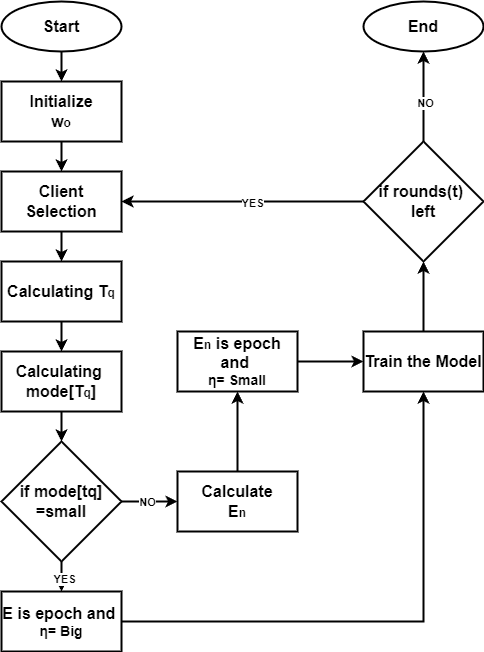
\includegraphics[scale=.28]{Images/Result Images/Flow_FedLR }
	\caption{Flow Chart describing the workings of FedFL.}
	\label{FlowFedLR}
\end{figure}
Fig. \ref{FlowFedLR} shows the workings of FedLR. Initialize the global parameter value $w_0$.Selection of all the eligible clients for training.Finding each client’s run-time as they finish training. Finding the mode time value by comparing the individual times. Selecting the learning rate and epoch values based on the mode value. The bigger learning rate ($\eta$) will be assigned to quicker devices with the default epoch ($E$) value. The slacker devices will be assigned a lower learning rate with a lower epoch value En using equation \ref{eq1}. and a smaller $\eta$. The time of these devices will be compared next, and the
slacker devices will receive a low amount of work but will still be a pivotal element in the federated learning process.

\section{Result and Analysis}
The model architecture used in the experiments is a 2 layered Convolution Neural Network. The list of datasets used for the experiments are as follows:
\begin{enumerate}
    \item CIFAR10 \cite{cifar10} dataset containing ten classes.
    \item MNIST \cite{lecun1998mnist} dataset of Handwritten digits containing ten classes. 
    \item FMNIST \cite{xiao2017fashionmnistnovelimagedataset} dataset of fashion items containing ten classes.
    \item CIFAR100 \cite{Krizhevsky09learningmultiple} dataset containing hundred classes. 
\end{enumerate}
\subsection{Machines Used}
Two machines are used to test the proposed algorithm, and the specifications of the machines are given below:
\begin{enumerate}
	\item Google Collab (Free Tier with T4 GPU).
	\item Workstation (128GB RAM, Intel Xeon Silver 4216 CPU, and NVIDIA RTX A4000 GPU)
\end{enumerate}

All clients use the full datasets and run at 10 Epochs and 10 Communication Rounds. Using .25 and 1 GPU and CPU, respectively in Flower. The Results of our Experiments are as follows:
10 Clients using FedAvg, FedProx, and FedLR on all Datasets. The blue dotted lines represent the local loss and accuracy, while the orange ones represent the global loss and accuracy. The legends show how many total epochs one client takes.

%\begin{figure}[htp!]
%	\centering
%	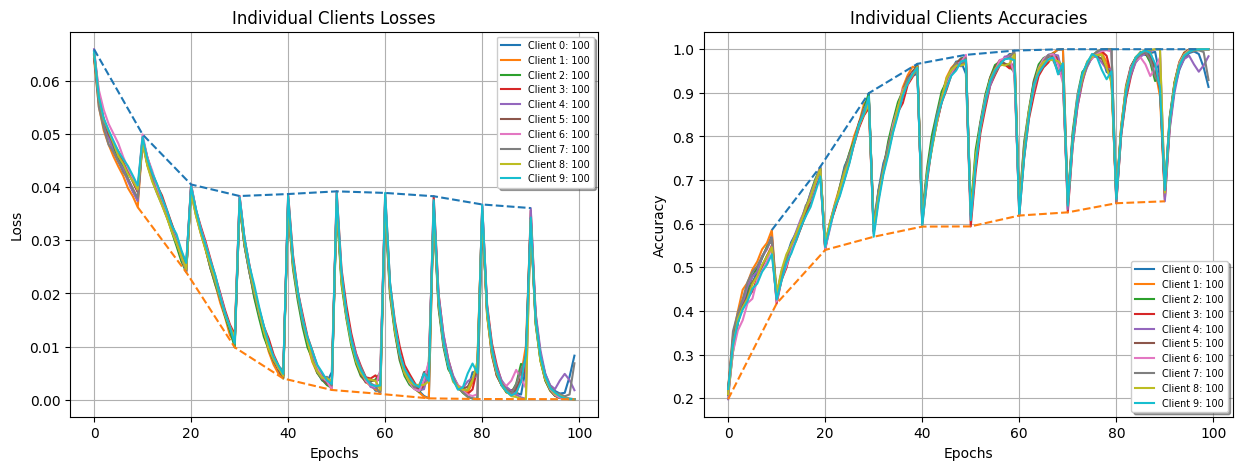
\includegraphics[scale=.28]{Images/Result Images/CIFAR 10/cifar10_fedavg_lossacc }
%	\caption{Accuracy and Loss of 10 Clients using FedAvg on the CIFAR10 Dataset (Workstation).}
%	\label{FedAvgC10}
%\end{figure}
%
%\begin{figure}[htp!]
%	\centering
%	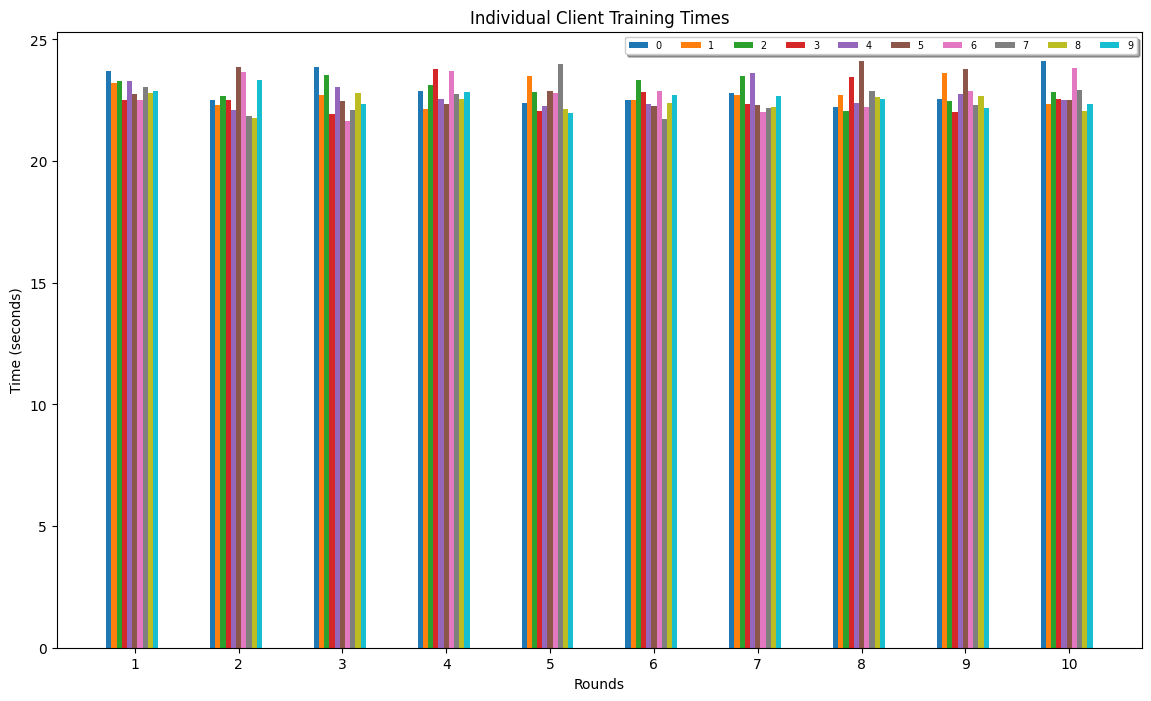
\includegraphics[scale=.3]{Images/Result Images/CIFAR 10/cifar10_fedavg_total_time_635o65 }
%	\caption{Individual Time of 10 Clients using FedAvg on the CIFAR10 Dataset (Workstation).}
%	\label{FedAvgTimeC10}
%\end{figure}
\begin{figure}[htp!]
	\centering
	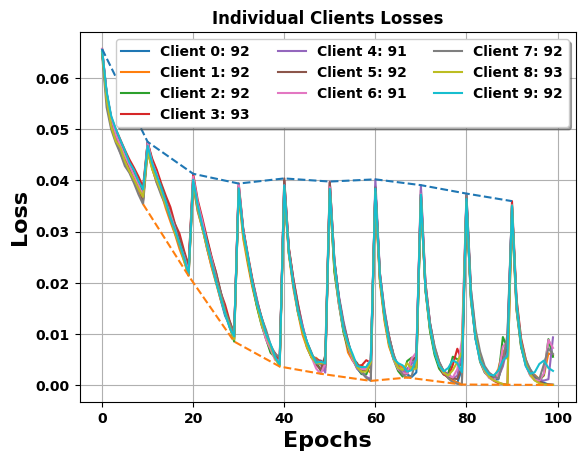
\includegraphics[scale=.51]{Images/NEWGRAPHS/loss_fedavg.png }
	\caption{Loss of 10 Clients using FedAvg on the CIFAR10 Dataset (Workstation).}
	\label{lossFedAvgC10}
\end{figure}

\begin{figure}[htp!]
	\centering
	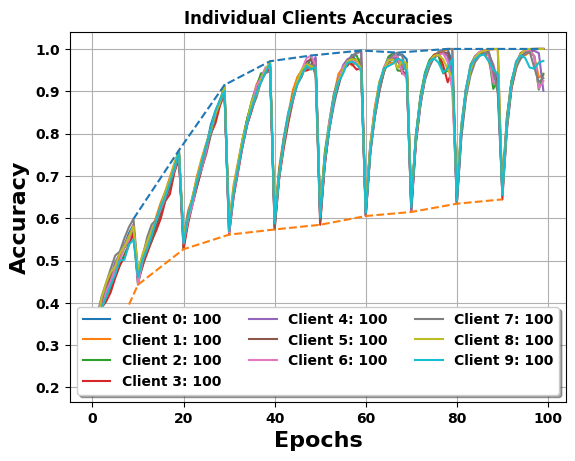
\includegraphics[scale=.51]{Images/NEWGRAPHS/acc_fedavg.png }
	\caption{Accuracy of 10 Clients using FedAvg on the CIFAR10 Dataset (Workstation).}
	\label{accFedAvgC10}
\end{figure}

\begin{figure}[htp!]
	\centering
	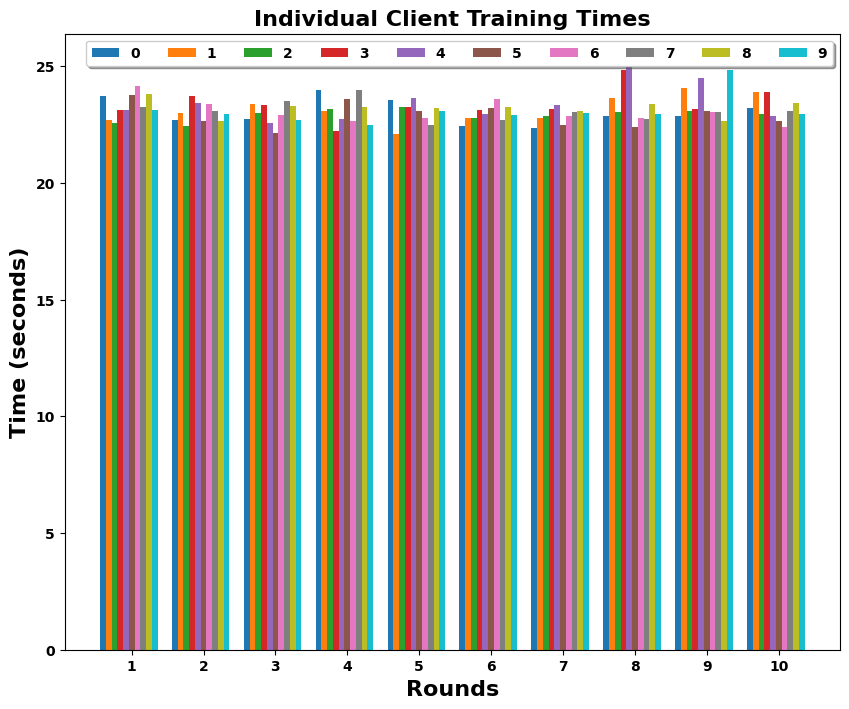
\includegraphics[scale=.4]{Images/NEWGRAPHS/time_fedavg_647o56.png }
	\caption{Individual Time of 10 Clients using FedAvg on the CIFAR10 Dataset (Workstation).}
	\label{FedAvgTimeC10}
\end{figure}


Fig. \ref{lossFedAvgC10}, \ref{accFedAvgC10} and \ref{FedAvgTimeC10} represent the loss, accuracy, and Individual time taken by each client, respectively, for FedAvg.  These are workstation times and the accuracy and losses are similar to FedLR and FedProx. The blue dotted lines represent the local loss and accuracy, while the orange ones represent the global loss and accuracy. The legend of the fig. \ref{lossFedAvgC10} shows how many total epochs one client takes.

Fig. \ref{lossFedProxC10}, \ref{accFedProxC10} and \ref{FedProxTimeC10} represent the loss, accuracy, and Individual time taken by each client, respectively, for FedProx. FedProx performs a bit better in terms of total communication cost than FedAvg in some scenarios.
%\begin{figure}[htp!]
%	\centering
%	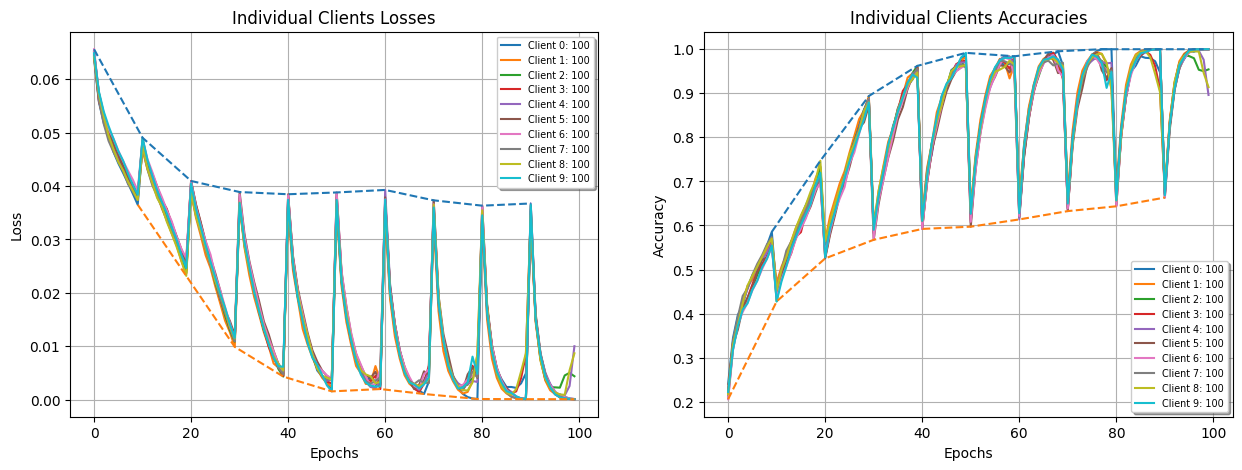
\includegraphics[scale=.28]{Images/Result Images/CIFAR 10/cifar10_fedPROX_lossacc }
%	\caption{Accuracy and Loss of 10 Clients using FedProx on the CIFAR10 Dataset (Workstation).}
%	\label{FedProxC10}
%\end{figure}
%
%\begin{figure}[htp!]
%	\centering
%	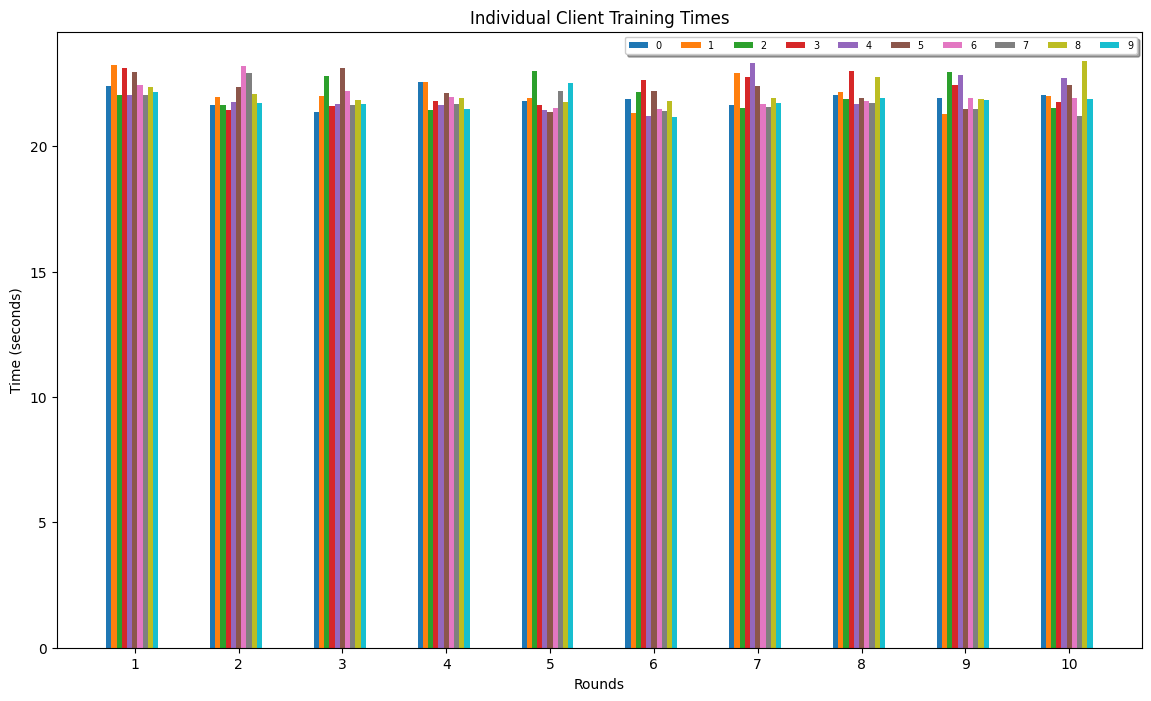
\includegraphics[scale=.3]{Images/Result Images/CIFAR 10/cifar10_fedPROX_total_time_622o28 }
%	\caption{Individual Time of 10 Clients using FedProx on the CIFAR10 Dataset (Workstation).}
%	\label{FedProxTimeC10}
%\end{figure}

\begin{figure}[htp!]
	\centering
	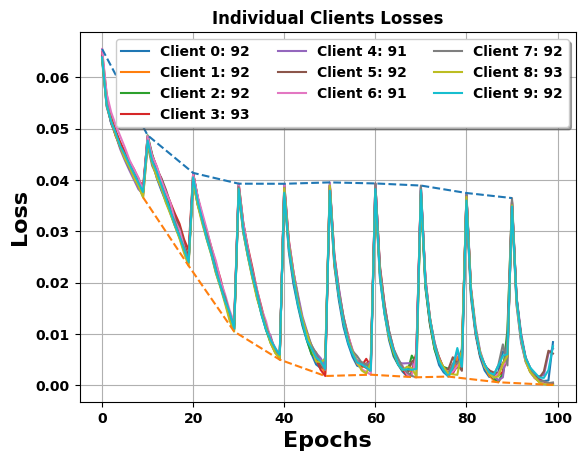
\includegraphics[scale=.51]{Images/NEWGRAPHS/loss_fedprox.png }
	\caption{Loss of 10 Clients using FedProx on the CIFAR10 Dataset (Workstation).}
	\label{lossFedProxC10}
\end{figure}

\begin{figure}[htp!]
	\centering
	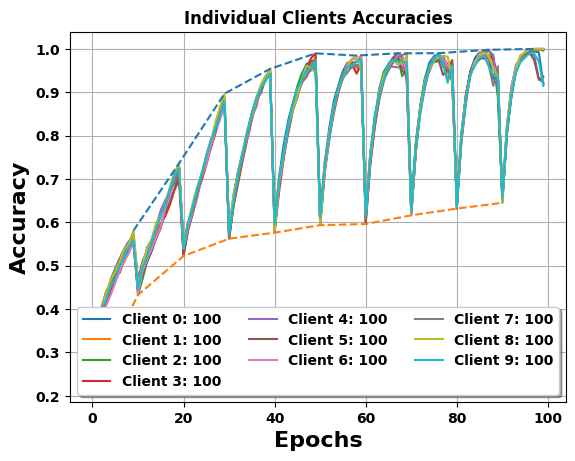
\includegraphics[scale=.51]{Images/NEWGRAPHS/acc_fedprox.png }
	\caption{Accuracy of 10 Clients using FedProx on the CIFAR10 Dataset (Workstation).}
	\label{accFedProxC10}
\end{figure}


\begin{figure}[htp!]
	\centering
	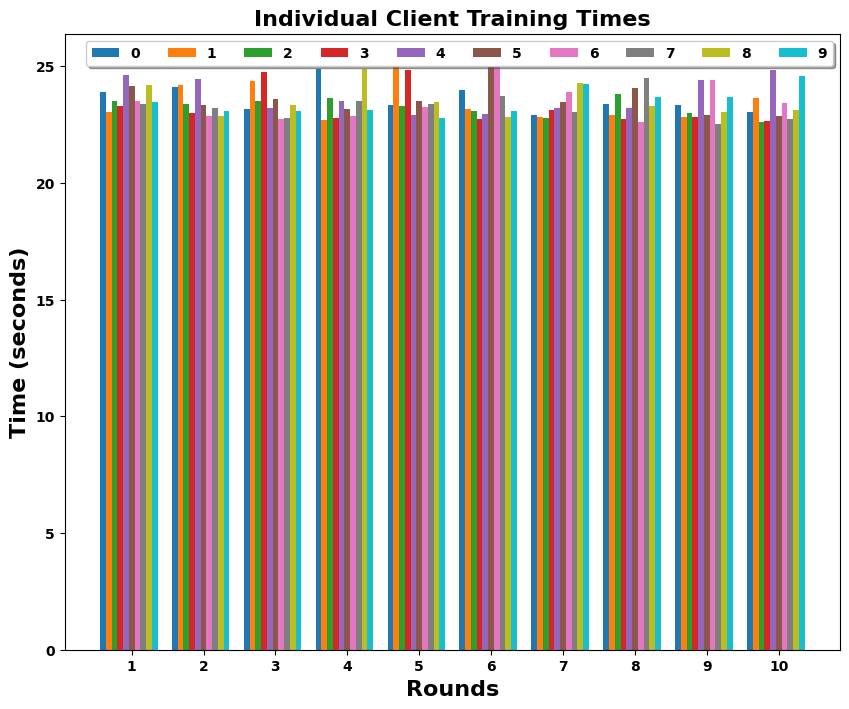
\includegraphics[scale=.4]{Images/NEWGRAPHS/time_fedprox_653o8.png }
	\caption{Individual Time of 10 Clients using FedProx on the CIFAR10 Dataset (Workstation).}
	\label{FedProxTimeC10}
\end{figure}


%\begin{figure}[htp!]
%	\centering
%	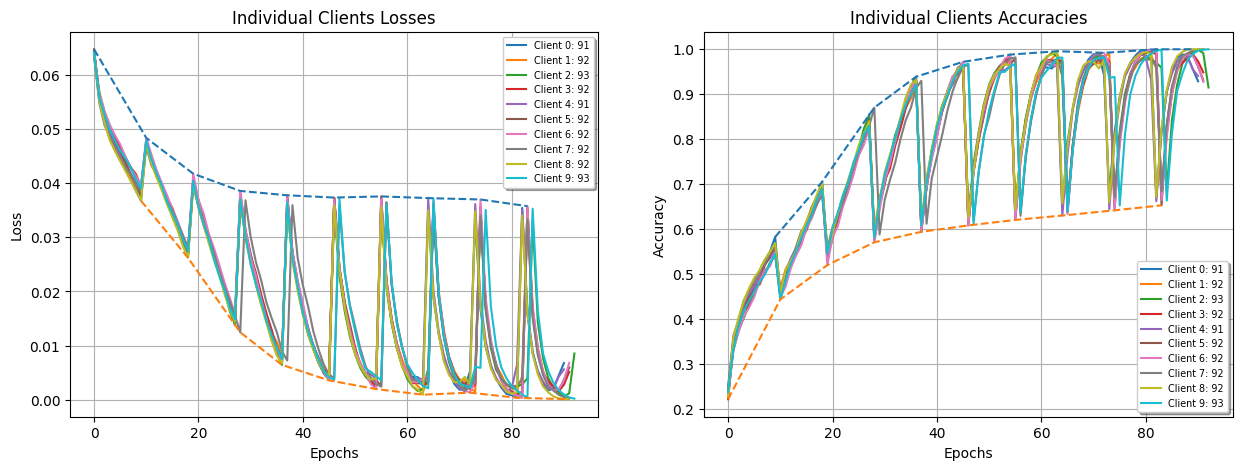
\includegraphics[scale=.28]{Images/Result Images/CIFAR 10/cifar10_mystrat_lossacc }
%	\caption{Accuracy and Loss of 10 Clients using FedLR on the CIFAR10 Dataset (Workstation).}
%	\label{FedLRC10}
%\end{figure}
%
%\begin{figure}[htp!]
%	\centering
%	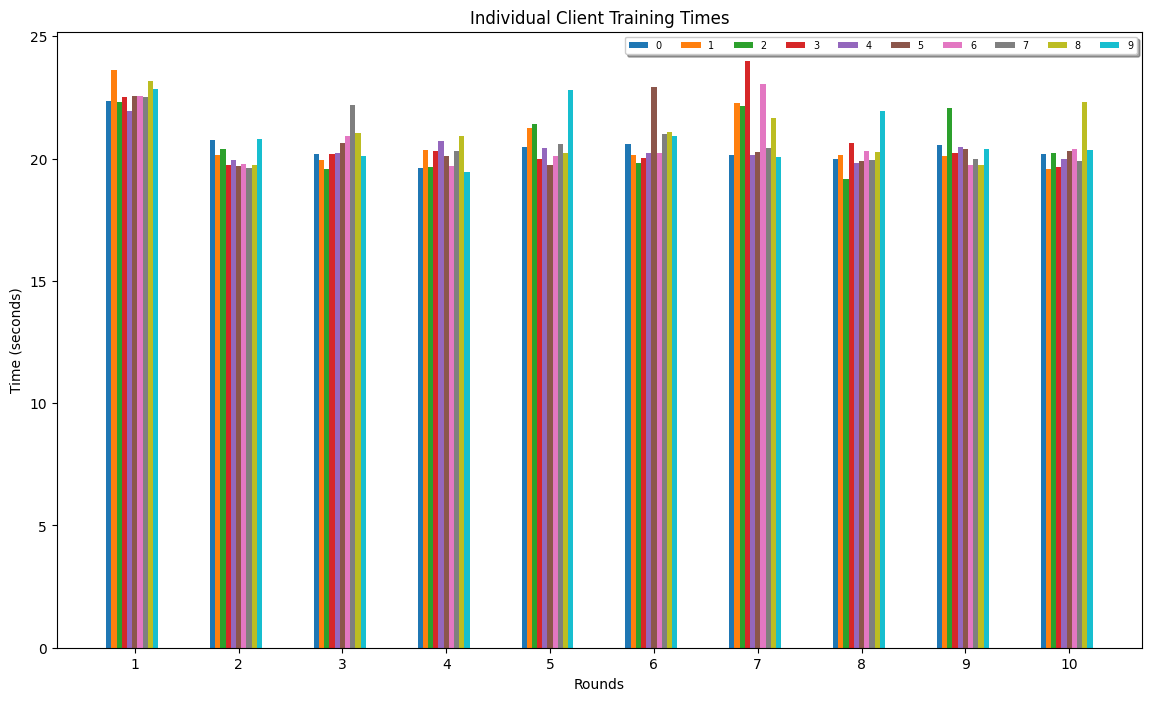
\includegraphics[scale=.3]{Images/Result Images/CIFAR 10/cifar10_total_time_589o74 }
%	\caption{Individual Time of 10 Clients using FedLR on the CIFAR10 Dataset (Workstation).}
%	\label{FedLRTimeC10}

\begin{figure}[htp!]
	\centering
	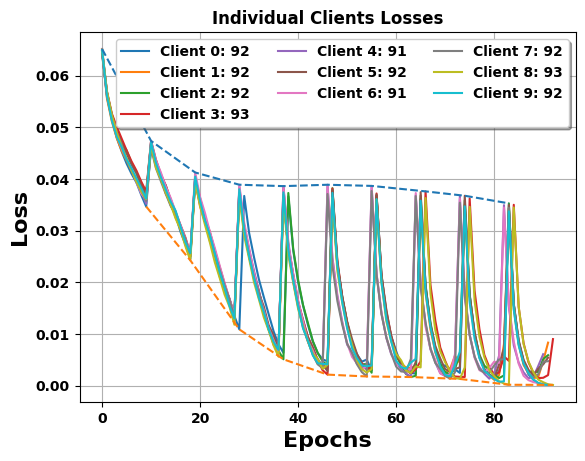
\includegraphics[scale=.51]{Images/NEWGRAPHS/loss_fedlr.png}
	\caption{Loss of 10 Clients using FedLR on the CIFAR10 Dataset (Workstation).}
	\label{lossFedLRC10}
\end{figure}

\begin{figure}[htp!]
	\centering
	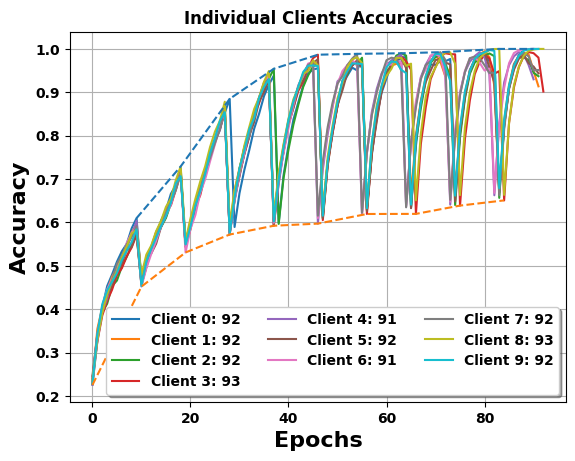
\includegraphics[scale=.51]{Images/NEWGRAPHS/acc_fedlr.png}
	\caption{Accuracy of 10 Clients using FedLR on the CIFAR10 Dataset (Workstation).}
	\label{accFedLRC10}
\end{figure}

\begin{figure}[htp!]
	\centering
	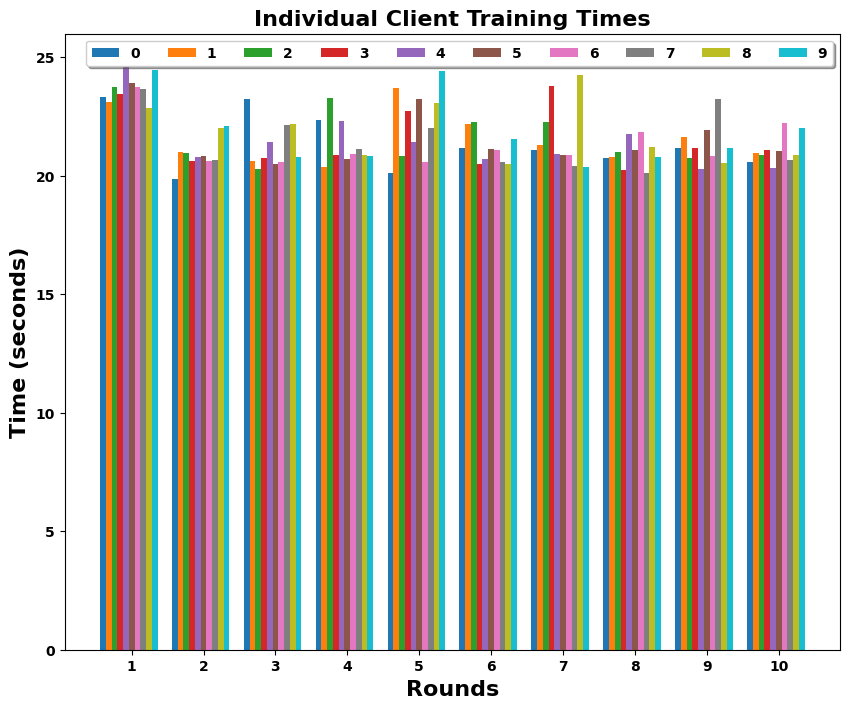
\includegraphics[scale=.4]{Images/NEWGRAPHS/time_fedlr_612o83.png}
	\caption{Individual Time of 10 Clients using FedLR on the CIFAR10 Dataset (Workstation).}
	\label{FedLRTimeC10}


\end{figure}
Fig. \ref{lossFedLRC10},\ref{accFedLRC10} and \ref{FedLRTimeC10} represent the loss, accuracy,
and Individual time taken by each client respectively for FedLR. In fig. \ref{lossFedLRC10}, each client runs a different number of epochs. The ones with the lowest epochs are the Slacker devices; hence, they contributed less. It is to be noted that the resources of each client are given at random to promote heterogeneity. Hence, none of the clients completed 100 $E$ due to them being slackers in a few rounds.

\begin{figure}[htp!]
	\centering
	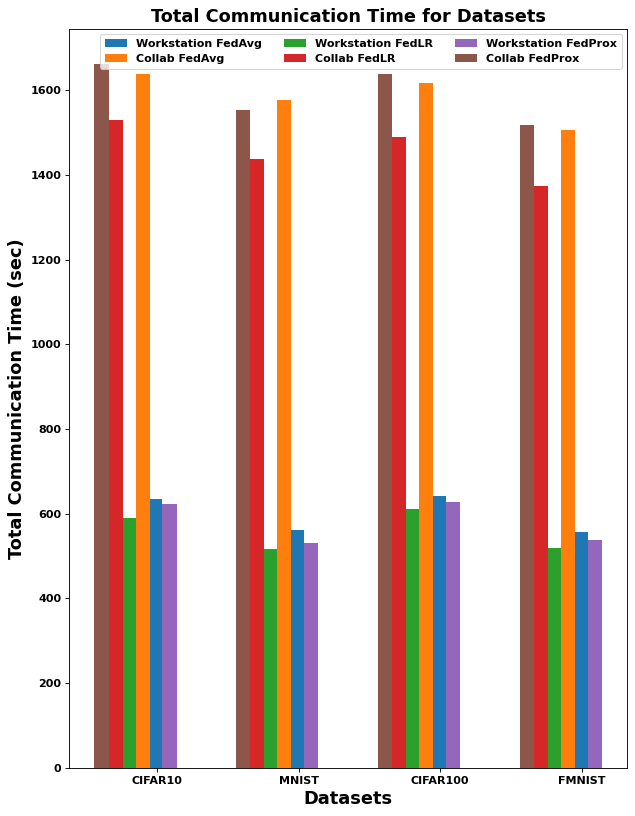
\includegraphics[scale=.4]{Images/Result Images/FinalGraphwithFedprox }
	\caption{Total Communication Time for Datasets.}
	\label{Finalgraph}
\end{figure}


Fig \ref{accFedAvgC10}, \ref{accFedLRC10}, and \ref{accFedProxC10} all show similar accuracy. This same pattern is seen in other datasets as well \cite{lecun1998mnist}  \cite{xiao2017fashionmnistnovelimagedataset} \cite{Krizhevsky09learningmultiple}. But fig \ref{FedAvgTimeC10}, \ref{FedProxTimeC10}, and \ref{FedLRTimeC10} shows the total individual times of each client, which is smallest in the case of FedLR. The detailed results can be found in table \ref{totaltimetable} and the visual representation in fig. \ref{Finalgraph}. In all the workstation results, FedLR has shown the best results, and FedProx is the second best. But in collab results, it was a mixed bag. As Collab gives you a random T4 GPU in each instance, which means the heterogeneity is more severe. Which lead to FedAvg performing better than FedProx in some cases.
% Please add the following required packages to your document preamble:
% \usepackage{multirow}
% \usepackage{graphicx}
\begin{table}[ht]
	\centering
	\caption{Total Communication Time with Different Datasets }
	\resizebox{\columnwidth}{!}{%
		\begin{tabular}{|l|l|l|l|l|}
			\hline
			Datasets                  & System      & FedLR (sec) & FedAvg (sec) & FedProx (sec) \\ \hline
			\multirow{2}{*}{CIFAR10}  & Workstation & 612.83      & 647.56       & 653.80        \\ \cline{2-5} 
			& Collab      & 1528.82     & 1638.73      & 1662.25       \\ \hline
			\multirow{2}{*}{MNIST}    & Workstation & 515.81      & 562.51       & 531.81        \\ \cline{2-5} 
			& Collab      & 1438.09     & 1576.74      & 1553.16       \\ \hline
			\multirow{2}{*}{CIFAR100} & Workstation & 611.08      & 641.14       & 628.44        \\ \cline{2-5} 
			& Collab      & 1490.00     & 1617.62      & 1637.13       \\ \hline
			\multirow{2}{*}{FMNIST}   & Workstation & 519.84      & 557.56       & 537.23        \\ \cline{2-5} 
			& Collab      & 1374.31     & 1504.77      & 1516.53       \\ \hline
		\end{tabular}%
	}\label{totaltimetable}
\end{table}
To interpret the results more easily Percentage difference has been calculated. Comparison between FedLR and FedAvg as well as FedLR and FedProx. Table \ref{percentage_table} shows the detailed results. In the workstation setting, the proposed methodology has performed better than FedAvg and FedProx. However. as we have explained earlier, in the case of Google Collab, the results were a bit different. All tests have been run several times, and the full results are available at Github \cite{gitflwr}.
% Please add the following required packages to your document preamble:
% \usepackage{graphicx}
\begin{table}[ht]
	\centering
	\caption{Percentage Difference of Communication Time with Different Datasets }
	\resizebox{\columnwidth}{!}{%
		\begin{tabular}{|l|l|l|l|l|}
			\hline
			Datasets & \begin{tabular}[c]{@{}l@{}}Workstation\\ FedAvg\end{tabular} & \begin{tabular}[c]{@{}l@{}}Collab\\ FedAvg\end{tabular} & \begin{tabular}[c]{@{}l@{}}Workstation\\ FedProx\end{tabular} & \begin{tabular}[c]{@{}l@{}}Collab\\ FedProx\end{tabular} \\ \hline
			CIFAR10  & 5.5\%                                                         & 6.9\%                                                    & 6.4\%                                                          & 8.3\%                                                     \\ \hline
			MNIST    & 8.7\%                                                         & 9.2\%                                                    & 3\%                                                            & 7.7\%                                                     \\ \hline
			CIFAR100 & 4.8\%                                                         & 8.2\%                                                    & 2.8\%                                                          & 9.4\%                                                     \\ \hline
			FMNIST   & 7.0\%                                                           & 9.0\%                                                    & 3.3\%                                                          & 9.8\%                                                     \\ \hline
		\end{tabular}%
	}\label{percentage_table}
\end{table}



\section{Conclusion}
The proposed algorithm has reduced the total communication time by a significant margin and has maintained fairness in the system while maintaining the accuracy of the models. The proposed algorithm has also been tested on two different devices to prove the improvements in communication rounds for a federated learning system with many slacker devices. The two devices prove the heterogeneity aspect of the proposed system. Both FedAvg and FedProx are compared with the proposed work, and the proposed work has significantly improved over both of them. Using the proposed methodology in real-world IoT and Edge devices will make the Federated Learning process more efficient and robust.
\bibliographystyle{unsrt}
\bibliography{Sample}


\end{document}


